\section{Labelbox}
\noindent The subset of images from the FFHQ \cite{FFHQ} dataset was classified using Labelbox \cite{Labelbox}. Using the Slice \cite{LabelboxSlice} feature, we could batch-process data from multiple Datasets \cite{LabelboxDataset} and query with natural language. Exporting the filtered images produced a .ndjson file containing the image and augmented meta-data.\\
\begin{figure}[h!]
    \centering
    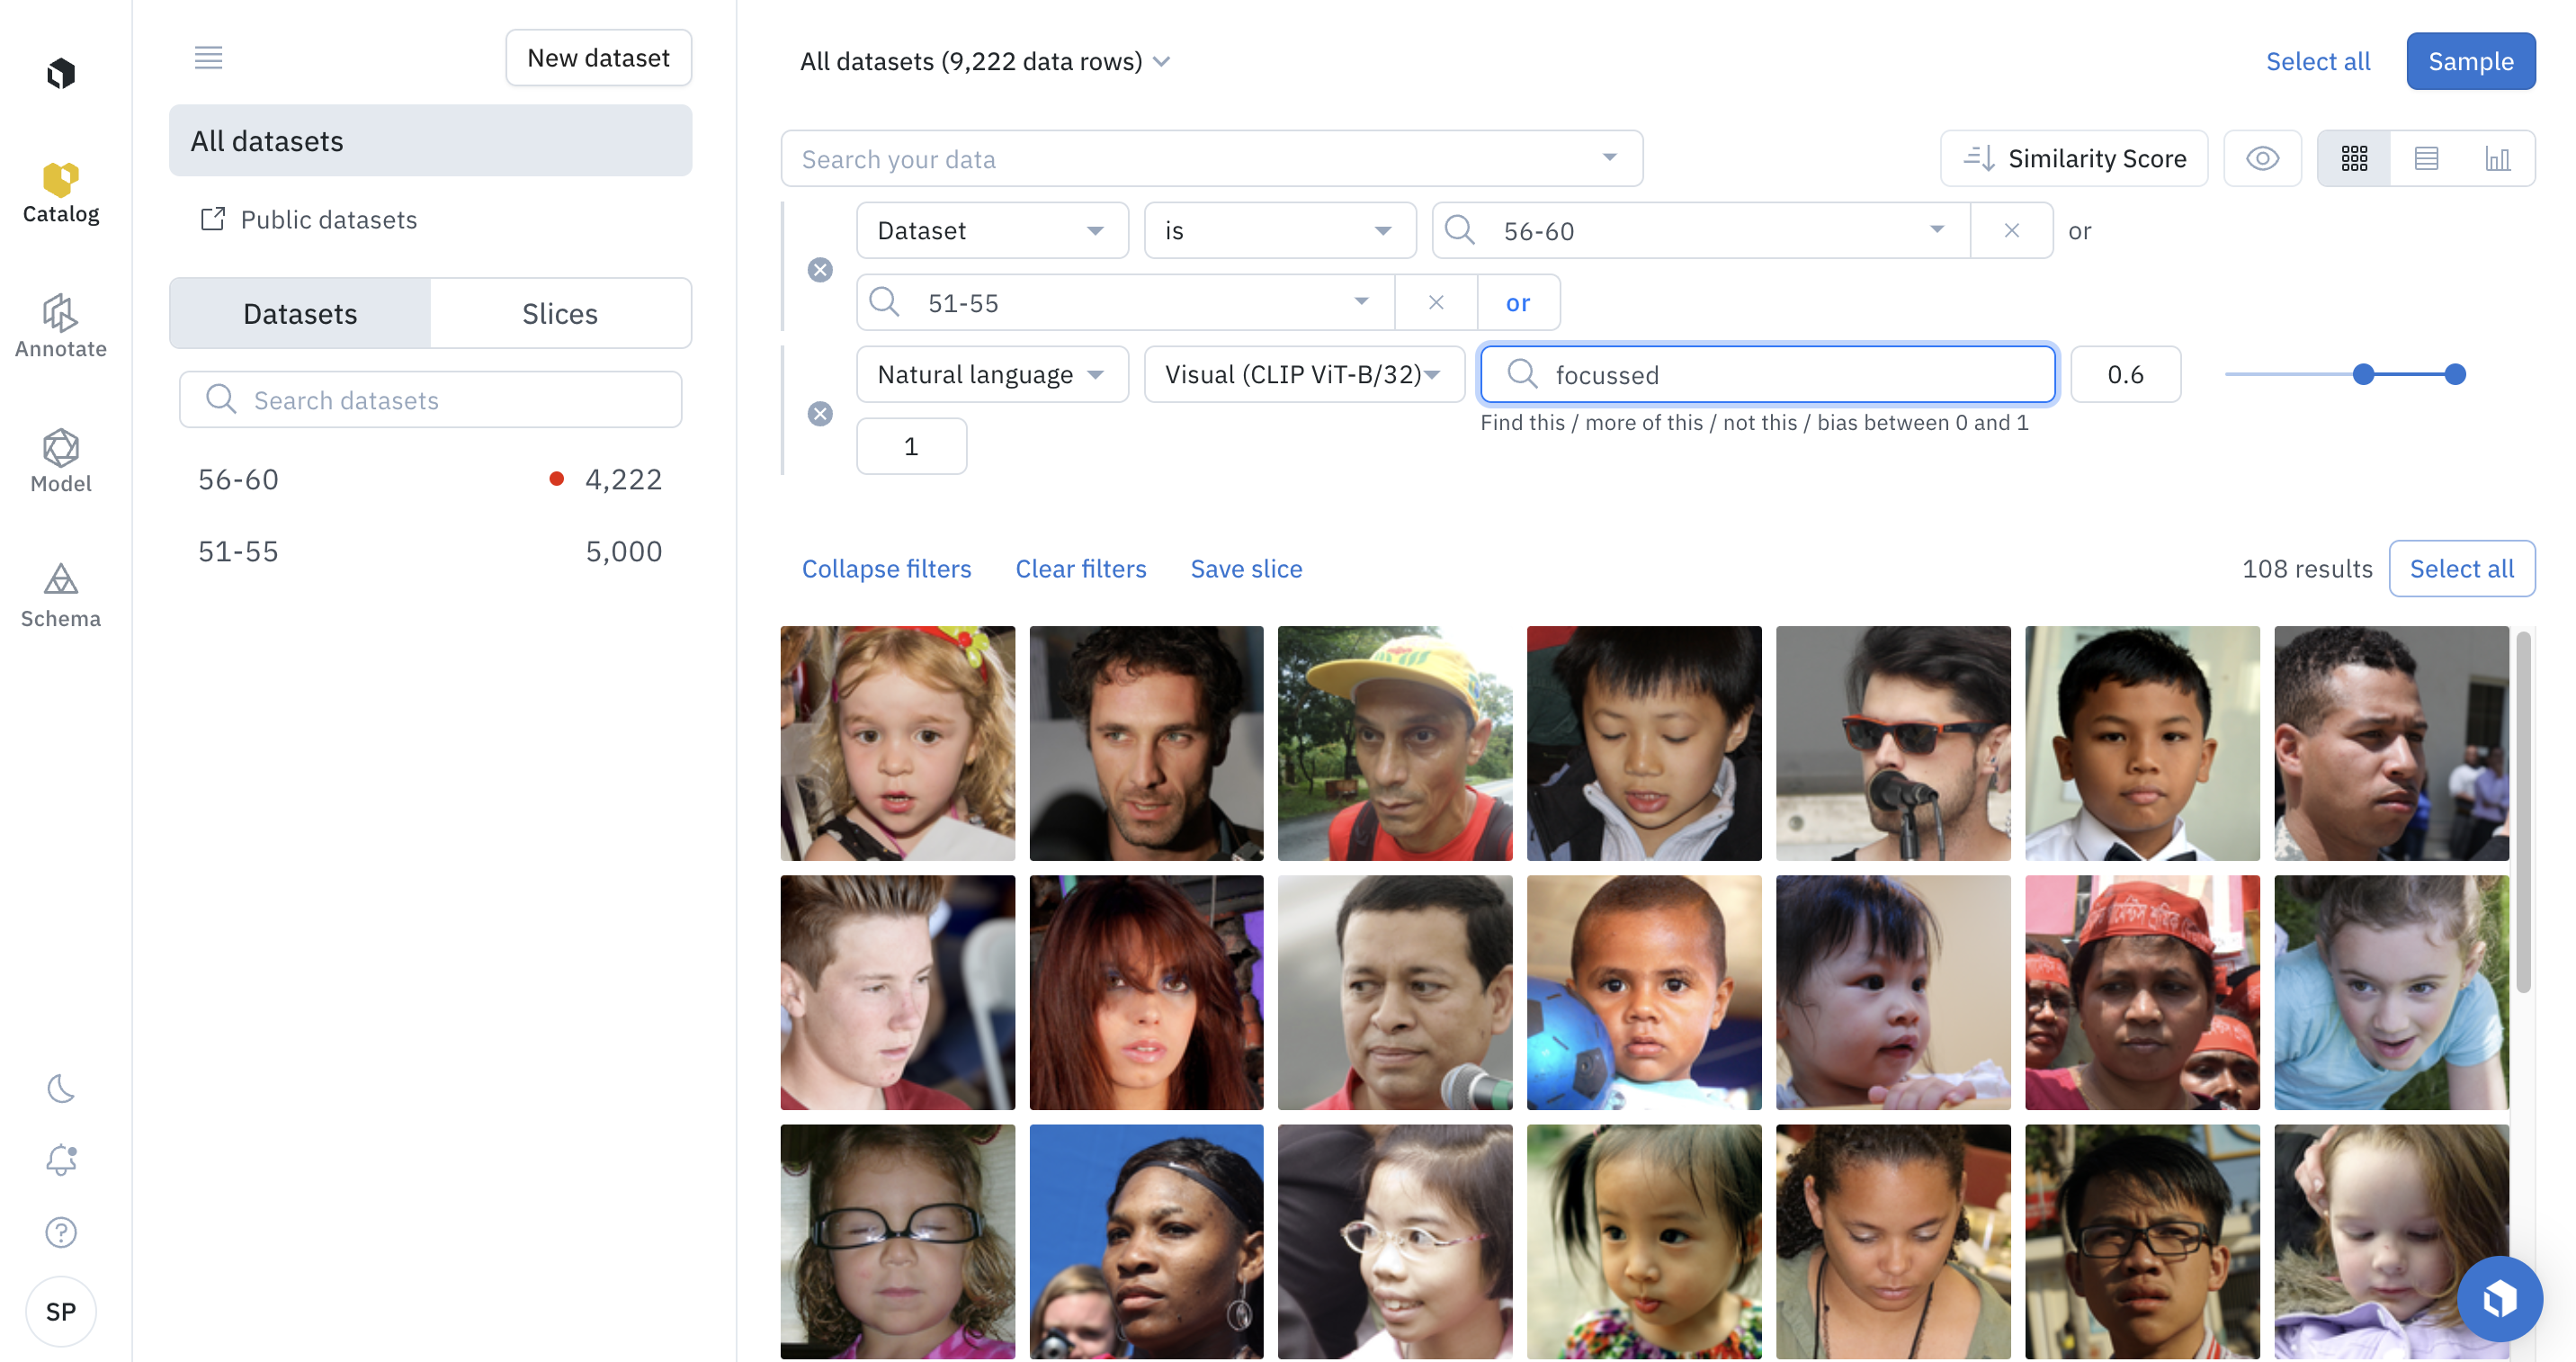
\includegraphics[width=\textwidth]{resources/labelbox.png}
    \caption{Labelbox \cite{Labelbox} Slice \cite{LabelboxSlice}}
\end{figure}


\section{Challages}

\noindent Once the images are filtered, Labelbox \cite{Labelbox} exports a JSON file containing the image and its metadata attributes. A Python script helped consolidate the filtered images from each data row in the .ndjson file.\\

\lstdefinestyle{json}{
  basicstyle=\ttfamily,
  numbers=left,
  numberstyle=\small,
  numbersep=5pt,
  breaklines=true,
  frame=single,
  backgroundcolor=\color{white},  % Set background color to white
  language=Python,
  showstringspaces=false,
  keywordstyle=\color{blue},
  commentstyle=\color{green},
  stringstyle=\color{black},       % Set text color to black
  literate={\\}{{\char`\\}}1,
  captionpos=b
}

\begin{lstlisting}[style=json, caption={Sample .ndjson after exporting some filtered images using Labelbox \cite{Labelbox} Slice \cite{LabelboxSlice}}]
{
    "data_row": {
        "id": "clo6k6aga2vxn08148v3qzlcj",
        "external_id": "54447.png",
        "row_data": "https://storage.labelbox.com/clo5koike05730700hvpyczq3%2F7990c767-3eec-c078-2f3a-187822eac361-54447.png?Expires=1698374509407&KeyName=labelbox-assets-key-3&Signature=gft6u5XmfI0ungpTrQVnEt59pAA",
        "details": {
        "dataset_id": "clo6jz4u0003t07089x6qhags",
        "dataset_name": "51-55",
        "created_at": "2023-10-26T02:21:46.185+00:00",
        "updated_at": "2023-10-26T02:22:17.137+00:00",
        "last_activity_at": "2023-10-26T02:21:46.000+00:00",
        "created_by": "sa_pra@live.concordia.ca"
        }
    },
    "media_attributes": {
        "height": 128,
        "width": 128,
        "mime_type": "image/png",
        "exif_rotation": "1"
    },
    "attachments": [],
    "metadata_fields": []
}      
\end{lstlisting}
\vspace*{1em}

\lstset{
  language=Python,
  basicstyle=\ttfamily,
  numbers=left,
  frame=single,
  captionpos=b,
}

\begin{lstlisting}[caption={Consolidating the images}]
with open(ndjson_file_path, 'r') as ndjson_file:
    for index, line in enumerate(ndjson_file, start=1):
        try:
            data = json.loads(line)
            image_url = data['data_row']['row_data']

            image_filename = os.path.join(
                save_directory, f'focus_{index:04d}.png'
            )

            response = requests.get(image_url)
            if response.status_code == 200:
                with open(image_filename, 'wb') as f:
                    f.write(response.content)
                print(f"Image saved as {image_filename}")
        
        except json.JSONDecodeError as e:
            print(f"DecodeError: {e}")
        
        except KeyError as e:
            print(f"KeyError: {e}")
\end{lstlisting}